\documentclass[border=15pt]{standalone}
%%%<
\usepackage{verbatim}
%%%>
\begin{comment}
:Title: Filling the space below a surface plot
:Tags: 3D;Functions;Filling;fillbetween;colormaps
:Author: Stefan Kottwitz
:Slug: fill-space-3d

Here I fill the space below the function z = x^2+y^2 to get
a solid object. I did it by:

- Plotting the curves at the edges, for x=0 and y=0
- Plotting the bottom edges
- Naming the paths above using name path
- Using the fillbetween library to fill the space between top boundary curves and the bottom edges
- Defining a pgf layer for the background and plotting the original surface z = x^2+y^2 on it, so the boundary areas on the main layer hide parts of the function
- Shading the boundary areas improve the 3D look

My oringinal post on TeXwelt.de: http://texwelt.de/wissen/fragen/8690/
\end{comment}
\usepackage{pgfplots}
\usepgfplotslibrary{colormaps,fillbetween}
\pgfplotsset{compat=1.10}
\begin{document}
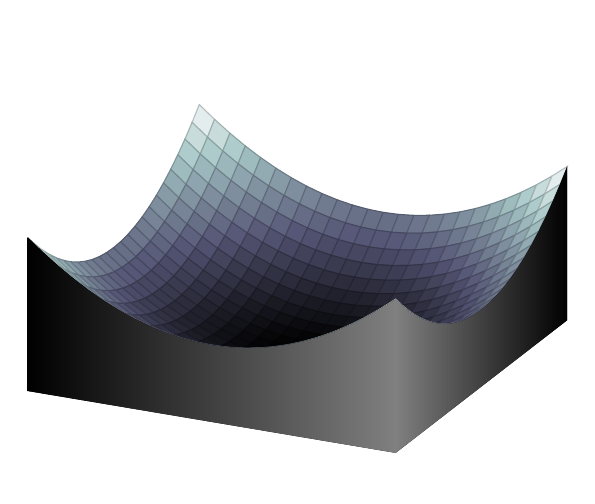
\begin{tikzpicture}
  \pgfdeclarelayer{pre main}
  \pgfsetlayers{pre main,main}
  \begin{axis}[
      hide axis,
      domain = -4:4,
      zmax   = 12,
      colormap/bone
    ]
    \begin{pgfonlayer}{pre main}
      \addplot3 [surf] {(x^2+y^2)/4};
    \end{pgfonlayer}
    \addplot3 [name path = xline, draw = none] (x,-4,0);
    \addplot3 [name path = yline, draw = none] (4,y,0);
    \addplot3 [name path = xcurve, y domain = 0:0, draw = none]
      (x, -4, {(x^2+16)/4});
    \addplot3 [name path = ycurve, y domain = 0:0, draw = none]
      (4, x, {(16+x^2)/4});
    \addplot [left color = black, right color = black!50, draw = none]
      fill between[of = xcurve and xline];
    \addplot [left color = black!50, right color = black, draw = none]
      fill between[of = yline and ycurve, reverse = true];
  \end{axis}
\end{tikzpicture}
\end{document}